% Options for packages loaded elsewhere
\PassOptionsToPackage{unicode}{hyperref}
\PassOptionsToPackage{hyphens}{url}
\PassOptionsToPackage{dvipsnames,svgnames,x11names}{xcolor}
%
\documentclass[
  letterpaper,
  DIV=11,
  numbers=noendperiod]{scrartcl}

\usepackage{amsmath,amssymb}
\usepackage{iftex}
\ifPDFTeX
  \usepackage[T1]{fontenc}
  \usepackage[utf8]{inputenc}
  \usepackage{textcomp} % provide euro and other symbols
\else % if luatex or xetex
  \usepackage{unicode-math}
  \defaultfontfeatures{Scale=MatchLowercase}
  \defaultfontfeatures[\rmfamily]{Ligatures=TeX,Scale=1}
\fi
\usepackage{lmodern}
\ifPDFTeX\else  
    % xetex/luatex font selection
\fi
% Use upquote if available, for straight quotes in verbatim environments
\IfFileExists{upquote.sty}{\usepackage{upquote}}{}
\IfFileExists{microtype.sty}{% use microtype if available
  \usepackage[]{microtype}
  \UseMicrotypeSet[protrusion]{basicmath} % disable protrusion for tt fonts
}{}
\makeatletter
\@ifundefined{KOMAClassName}{% if non-KOMA class
  \IfFileExists{parskip.sty}{%
    \usepackage{parskip}
  }{% else
    \setlength{\parindent}{0pt}
    \setlength{\parskip}{6pt plus 2pt minus 1pt}}
}{% if KOMA class
  \KOMAoptions{parskip=half}}
\makeatother
\usepackage{xcolor}
\setlength{\emergencystretch}{3em} % prevent overfull lines
\setcounter{secnumdepth}{-\maxdimen} % remove section numbering
% Make \paragraph and \subparagraph free-standing
\ifx\paragraph\undefined\else
  \let\oldparagraph\paragraph
  \renewcommand{\paragraph}[1]{\oldparagraph{#1}\mbox{}}
\fi
\ifx\subparagraph\undefined\else
  \let\oldsubparagraph\subparagraph
  \renewcommand{\subparagraph}[1]{\oldsubparagraph{#1}\mbox{}}
\fi


\providecommand{\tightlist}{%
  \setlength{\itemsep}{0pt}\setlength{\parskip}{0pt}}\usepackage{longtable,booktabs,array}
\usepackage{calc} % for calculating minipage widths
% Correct order of tables after \paragraph or \subparagraph
\usepackage{etoolbox}
\makeatletter
\patchcmd\longtable{\par}{\if@noskipsec\mbox{}\fi\par}{}{}
\makeatother
% Allow footnotes in longtable head/foot
\IfFileExists{footnotehyper.sty}{\usepackage{footnotehyper}}{\usepackage{footnote}}
\makesavenoteenv{longtable}
\usepackage{graphicx}
\makeatletter
\def\maxwidth{\ifdim\Gin@nat@width>\linewidth\linewidth\else\Gin@nat@width\fi}
\def\maxheight{\ifdim\Gin@nat@height>\textheight\textheight\else\Gin@nat@height\fi}
\makeatother
% Scale images if necessary, so that they will not overflow the page
% margins by default, and it is still possible to overwrite the defaults
% using explicit options in \includegraphics[width, height, ...]{}
\setkeys{Gin}{width=\maxwidth,height=\maxheight,keepaspectratio}
% Set default figure placement to htbp
\makeatletter
\def\fps@figure{htbp}
\makeatother
\newlength{\cslhangindent}
\setlength{\cslhangindent}{1.5em}
\newlength{\csllabelwidth}
\setlength{\csllabelwidth}{3em}
\newlength{\cslentryspacingunit} % times entry-spacing
\setlength{\cslentryspacingunit}{\parskip}
\newenvironment{CSLReferences}[2] % #1 hanging-ident, #2 entry spacing
 {% don't indent paragraphs
  \setlength{\parindent}{0pt}
  % turn on hanging indent if param 1 is 1
  \ifodd #1
  \let\oldpar\par
  \def\par{\hangindent=\cslhangindent\oldpar}
  \fi
  % set entry spacing
  \setlength{\parskip}{#2\cslentryspacingunit}
 }%
 {}
\usepackage{calc}
\newcommand{\CSLBlock}[1]{#1\hfill\break}
\newcommand{\CSLLeftMargin}[1]{\parbox[t]{\csllabelwidth}{#1}}
\newcommand{\CSLRightInline}[1]{\parbox[t]{\linewidth - \csllabelwidth}{#1}\break}
\newcommand{\CSLIndent}[1]{\hspace{\cslhangindent}#1}

\KOMAoption{captions}{tableheading}
\makeatletter
\makeatother
\makeatletter
\makeatother
\makeatletter
\@ifpackageloaded{caption}{}{\usepackage{caption}}
\AtBeginDocument{%
\ifdefined\contentsname
  \renewcommand*\contentsname{Table of contents}
\else
  \newcommand\contentsname{Table of contents}
\fi
\ifdefined\listfigurename
  \renewcommand*\listfigurename{List of Figures}
\else
  \newcommand\listfigurename{List of Figures}
\fi
\ifdefined\listtablename
  \renewcommand*\listtablename{List of Tables}
\else
  \newcommand\listtablename{List of Tables}
\fi
\ifdefined\figurename
  \renewcommand*\figurename{Figure}
\else
  \newcommand\figurename{Figure}
\fi
\ifdefined\tablename
  \renewcommand*\tablename{Table}
\else
  \newcommand\tablename{Table}
\fi
}
\@ifpackageloaded{float}{}{\usepackage{float}}
\floatstyle{ruled}
\@ifundefined{c@chapter}{\newfloat{codelisting}{h}{lop}}{\newfloat{codelisting}{h}{lop}[chapter]}
\floatname{codelisting}{Listing}
\newcommand*\listoflistings{\listof{codelisting}{List of Listings}}
\makeatother
\makeatletter
\@ifpackageloaded{caption}{}{\usepackage{caption}}
\@ifpackageloaded{subcaption}{}{\usepackage{subcaption}}
\makeatother
\makeatletter
\@ifpackageloaded{tcolorbox}{}{\usepackage[skins,breakable]{tcolorbox}}
\makeatother
\makeatletter
\@ifundefined{shadecolor}{\definecolor{shadecolor}{rgb}{.97, .97, .97}}
\makeatother
\makeatletter
\makeatother
\makeatletter
\makeatother
\ifLuaTeX
  \usepackage{selnolig}  % disable illegal ligatures
\fi
\IfFileExists{bookmark.sty}{\usepackage{bookmark}}{\usepackage{hyperref}}
\IfFileExists{xurl.sty}{\usepackage{xurl}}{} % add URL line breaks if available
\urlstyle{same} % disable monospaced font for URLs
\hypersetup{
  pdftitle={Hierarchical Bayesian regression modelling predicts biochemical rection energies and facilitates quantitative modelling of cell metabolism},
  pdfauthor={Teddy Groves; Nicholas Luke Cowie; Lars Keld Nielsen},
  colorlinks=true,
  linkcolor={blue},
  filecolor={Maroon},
  citecolor={Blue},
  urlcolor={Blue},
  pdfcreator={LaTeX via pandoc}}

\title{Hierarchical Bayesian regression modelling predicts biochemical
rection energies and facilitates quantitative modelling of cell
metabolism}
\author{Teddy Groves \and Nicholas Luke Cowie \and Lars Keld Nielsen}
\date{}

\begin{document}
\maketitle
\begin{abstract}
This paper presents Maud, a command-line application that implements
Bayesian statistical inference for kinetic models of biochemical
metabolic reaction networks. Maud takes into account quantitative
information from omics experiments and background knowledge, as well as
structural information about kinetic mechanisms, regulatory interactions
and enzyme knockouts. Below, we review the existing options in this
area, explain how Maud improves on the state of the art, describe the
intended modelling workflow and illustrate its use with an example
application.
\end{abstract}
\ifdefined\Shaded\renewenvironment{Shaded}{\begin{tcolorbox}[enhanced, breakable, sharp corners, interior hidden, borderline west={3pt}{0pt}{shadecolor}, boxrule=0pt, frame hidden]}{\end{tcolorbox}}\fi

\renewcommand*\contentsname{Table of contents}
{
\hypersetup{linkcolor=}
\setcounter{tocdepth}{3}
\tableofcontents
}
\hypertarget{introduction}{%
\section{Introduction}\label{introduction}}

A kinetic model of cellular metabolism aims to express what is known
about a cellular process in the form of an \emph{in silico}
representation of the underlying network of chemical reactions. Kinetic
models can be used to improve production of target molecules, determine
regulatory networks (Christodoulou et al. 2018) and identify potential
drug targets (DeBerardinis and Chandel 2016; Liberti et al. 2017).
However, the use of kinetic models in practice is hindered by their
dependence on noisy and uncertain information sources. Quantitative in
vivo measurements of chemical abundances, and in vitro measurements
relating to kinetic parameters, both contain vital information but are
notoriously inaccurate (REFERENCES). Practically useful kinetic
modelling therefore requires a principled statistical approach that
encompasses multiple possible model parameterisations.

Bayesian statistical inference can combine the structural information
implicit in kinetic models with knowledge about metabolic parameters and
information from omics measurements (P. A. Saa and Nielsen 2016;
Gopalakrishnan, Dash, and Maranas 2020). However, kinetic models pose
serious computational challenges for Bayesian inference (Gutenkunst et
al. 2007; A. Raue et al. 2010).

The scope of a kinetic model is defined by a stoichiometric matrix,
\(S\), in which rows represent metabolites, columns represent reactions,
and matrix elements \(s_{ij}\) represent the stoichiometric coefficient
of metabolite \(i\) in reaction \(j\). The change in metabolite
concentrations is

\begin{equation}\label{eq-1}
\frac{dC}{dt} = S\cdot v - \mu\cdot C 
\end{equation}

In equation \eqref{eq-1}, C represents a vector of metabolite
concentrations, \(v\) is a vector of reaction rates, and \(\mu\) is the
growth rate. The second term represents the dilution due to cell growth.

In a kinetic model, the rates, \(v\), are expressed as a function of the
enzyme concentrations, \(E\), the metabolite concentrations, \(C\), and
a set of parameters, \(\theta\) as shown in equation \eqref{eq-2}

\begin{equation}\label{eq-2}
v = f(C, E, \theta)
\end{equation}

The parameters must include sufficient boundary concentrations and
fluxes to solve \eqref{eq-1}.

It is common to assume pseudo-steady state for metabolites, i.e., the
rate of fluxes towards any metabolite is much greater than the rate of
change in concentration, \(𝑣 \gg \frac{𝑑𝐶}{𝑑𝑡}\). Moreover, the dilution
effect is assumed minimal, \(\mu\cdot C \ll \vec{v}\) (true unless the
concentration is very high). Finally, the enzyme concentration is
assumed constant for the period considered and hence part of the
parameters.

Given these assumptions and a set of values for \theta, a set of steady
state metabolite concentrations and fluxes can be found by solving for
\(C\) the algebraic equation:

\begin{equation}\label{eq-3}
S\cdot f(C;\theta) = 0
\end{equation}

In a fermentation context, \eqref{eq-3} captures the rapid kinetics
inside the cell, while another set of ODEs would be used to describe the
external substrate and product concentrations, which could act as
boundary parameters to \eqref{eq-3}.

In the context of kinetic modelling, Bayesian inference is appealing
because it allows uncertainty to be represented appropriately without
sacrificing mechanistic accuracy. Measurement uncertainty can naturally
be represented in a Bayesian measurement model, whereas the prior model
can represent quantitative uncertainty about kinetic parameters.
Finally, kinetic rate laws can be represented in Bayesian data
generation models with arbitrarily high fidelity. See (REFERENCES) for
more about Bayesian inference and (REFERENCE) for a discussion of
practical Bayesian workflow.

Another advantage is that Bayesian inference problems are well-posed
even when not all parameters are strongly identified. Sloppy models in
which measurable quantities are sensitive to combinations of parameters
but not to individual marginal parameter values are ubiquitous in models
of biological systems {[}gutenkunst\_2007; White et al. (2016){]}. The
parameter correlation structure represents the set of potential models
that describe the observed data. As we demonstrate in our case study
below, capturing this correlation structure is difficult outside a
Bayesian context.

Previous Bayesian kinetic models have either sacrificed mechanistic
accuracy or have attempted to fit realistic kinetic models using
obsolete or unreliable computational methods.

The most popular algorithm for fitting Bayesian statistical models is
Markov Chain Monte Carlo (MCMC). Modern MCMC algorithms allow
exploration of high- dimensional posterior distributions, have robust
failure diagnostics (Vehtari et al. 2021) and can incorporate fast
numerical solvers, thereby making inference feasible for Bayesian
kinetic models. Nonetheless, the kinetic modelling literature reports an
aversion to MCMC, rooted mainly in concerns about sampling time and the
presumed difficulty of implementing the required statistical model
(Andreas Raue et al. 2013; P. A. Saa and Nielsen 2016). We are only
aware of two recent attempts to implement a Bayesian kinetic modelling
approach using MCMC. Stapor et al. (2018) fitted detailed kinetic models
using relatively inefficient MCMC algorithms that do not scale well to
high dimensional parameter spaces limiting the scope of modelling.
Conversely, St. John et al. (2018) utilises an efficient sampling
algorithm but uses approximate kinetics, namely lin-log kinetics Visser
and Heijnen (2003), limiting the scope of interpreting parameters and
inferring cellular behaviour in experimental conditions outside the
reference dataset.

There have also been efforts to implement Bayesian inference for kinetic
models without the use of MCMC. Examples of alternative inference
methods include variational inference as in St. John et al. (2018),
rejection sampling and approximate Bayesian computation P. A. Saa and
Nielsen (2016) and Laplace approximation, in which the Fisher
information matrix is used to calculate a normal approximation around
the maximum a posteriori parameter configuration (Liebermeister and Noor
2021; Gopalakrishnan, Dash, and Maranas 2020; Stapor et al. 2018;
Andreas Raue et al. 2013). Non-MCMC-based Bayesian kinetic models have
limited utility because they lack reliable diagnostic tools for
verifying that their results approximate the target posterior
distribution. This is a problem because realistic kinetic models tend to
induce highly correlated, non-Gaussian, joint probability distributions
(Gutenkunst et al. 2007; Stapor et al. 2018).

Our application Maud is the first Bayesian kinetic model to combine
biologically realistic mechanistic accuracy---including accurate rate
laws, post- translational modification and thermodynamics---with fast,
robust MCMC sampling using adaptive Hamiltonian Monte Carlo. Further,
Maud is a general-purpose application that can be used to fit a wide
range of Bayesian kinetic models.

\hypertarget{results-and-discussion}{%
\section{Results and Discussion}\label{results-and-discussion}}

To demonstrate our application's capabilities, we used Maud to analyse
an artificial dataset based on the human methionine cycle. We first used
Maud to generate simulated training and validation measurements based on
plausible parameter values, then performed posterior sampling. Next, we
used Maud to predict the validation data.

To show that Maud is robust to missing measurements we compared the
results of fitting the full dataset with an intentionally incomplete
dataset. To demonstrate why a full Bayesian approach is preferable to an
approach based on a Laplace approximation of the posterior distribution,
we also fit our methionine cycle model using the latter method and
compared the results with MCMC sampling.

Finally, we investigated our results to find out what our model learned
about the contributions of different regulatory factors to the flux
through GNMT, an important reaction. This analysis illustrates how Maud
can be used to generate actionable insights about metabolism without the
need for further statistical analysis.

The methionine cycle, illustrated in
Figure~\ref{fig-methionine-reactions}, is a fundamental pathway in human
metabolism, whose intermediate metabolites participate in a variety of
mechanisms which must compete for the same resources. Due to this
competition, as well as the fact that all the functions occur
simultaneously, the methionine cycle is highly regulated, with 6 known
allosteric effectors (REFERENCE). This complex regulation means that
quantitative modelling of the methionine cycle requires a detailed
kinetic model: this is why we chose it as a case study for Maud.

\begin{figure}

{\centering 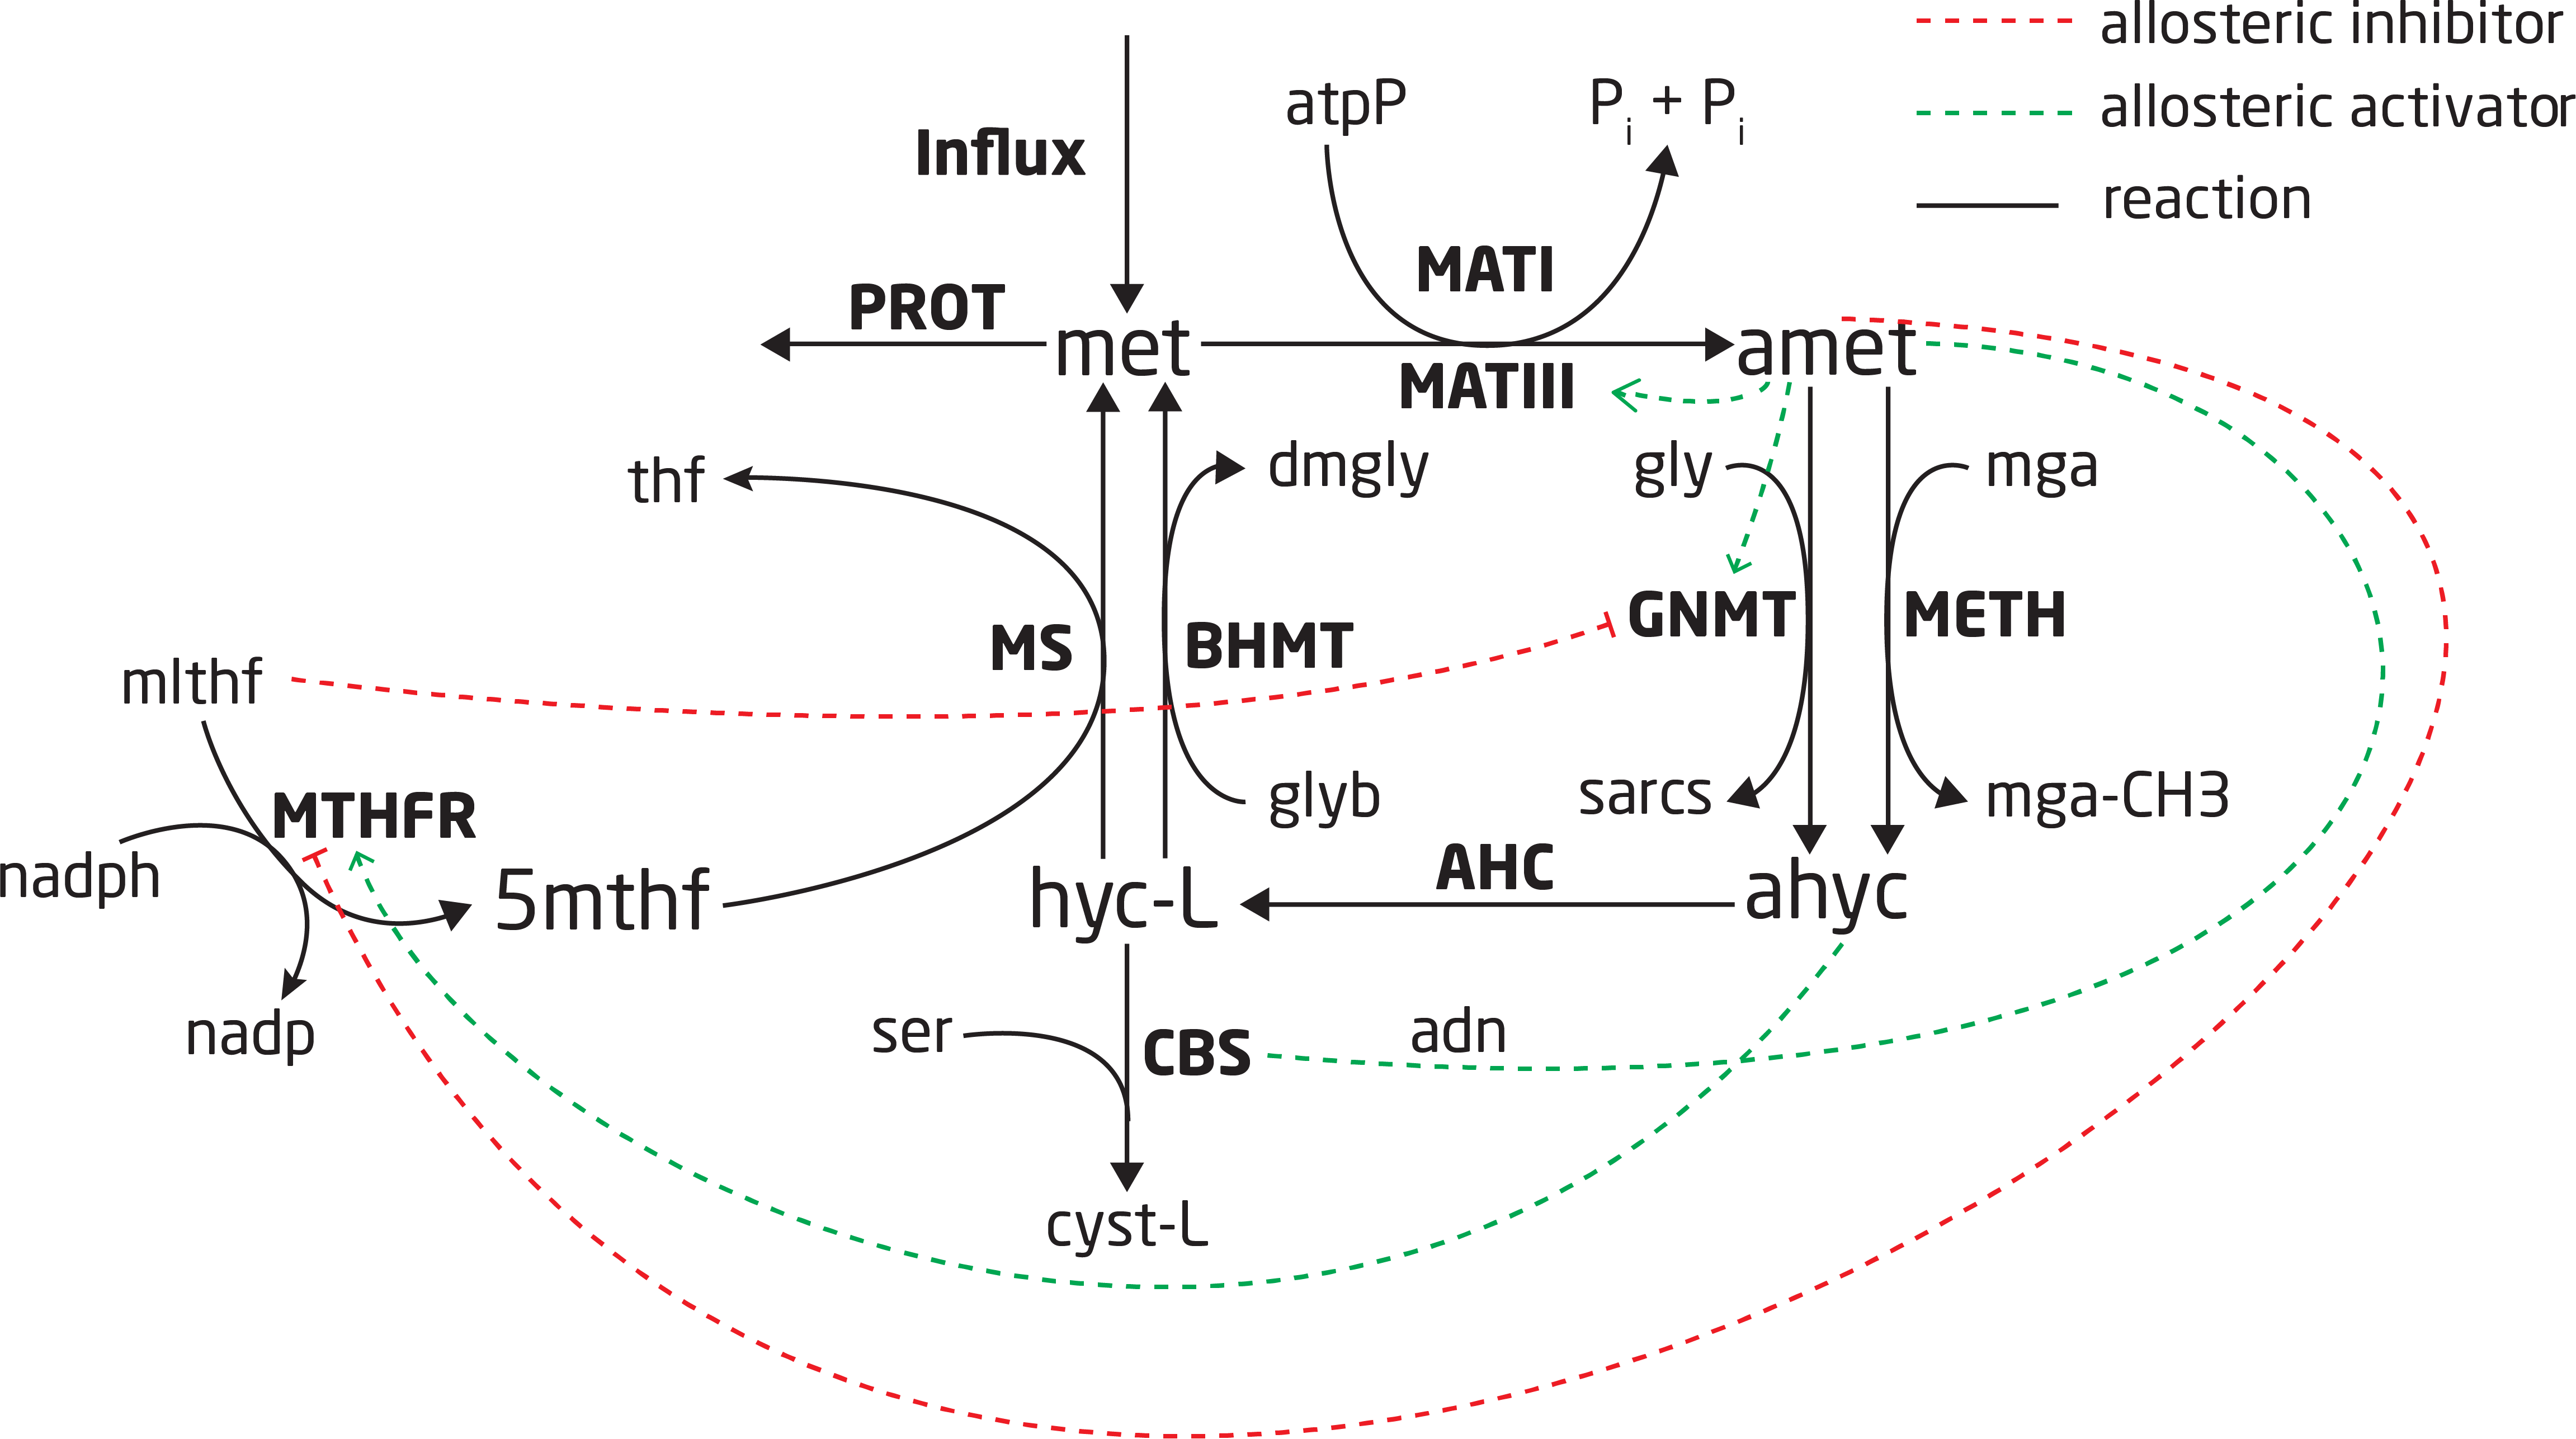
\includegraphics{./figures/methionine-reactions.png}

}

\caption{\label{fig-methionine-reactions}CAPTION - FILL THIS IN!}

\end{figure}

\hypertarget{dataset-and-model-specification}{%
\subsection{Dataset and model
specification}\label{dataset-and-model-specification}}

The simulated dataset and underlying kinetic model that we used for our
analysis can be found in {[}\#Supplementary Info{]}.

We constructed a kinetic model of the methionine cycle in Maud's format
using the description in Korendyaseva et al. (2008). The ordinary
differential equation system describing this model is shown in
Equation\,\eqref{eq-meth-ode}.

After specifying the qualitative aspects of the kinetic model, we chose
parameter values to use as ground truth by Monte Carlo sampling using a
previous model of the methionine cycle as a starting point (see P. Saa
and Nielsen (2015) for this model).

We used these parameters to simulate steady states in a range of
plausible experimental conditions, again using P. Saa and Nielsen (2015)
as a starting point. These steady states were then used to generate
simulated measurements using the measurement model described below.

\begin{equation}
a = b \label{eq-meth-ode}
\end{equation}

\hypertarget{measurement-model}{%
\subsubsection{Measurement model}\label{measurement-model}}

Generating an artificial dataset required a specification of the true
measurement error; we specified a standard deviation of 0.1 on
logarithmic scale for enzyme and metabolite concentration measurements,
corresponding to approximately 10\% measurement error and a standard
deviation for each reaction measurement approximately 10\% of the
simulated value.

These measurement error specifications are somewhat optimistic
considering the many sources of variation and uncertainty affecting
quantitative proteomics, metabolomics and fluxomics analyses, but are a
reasonable first approximation to a realistic set of measurements.

For our main model run, we assumed that all metabolite and enzyme
concentrations were measured, and that there was a reaction measurement
for each of the network's elementary flux modes.

\hypertarget{trainingvalidation-split}{%
\subsubsection{Training/validation
split}\label{trainingvalidation-split}}

The training testing split was selected to achieve a large difference
between the fluxes of the training and testing dataset. The split was
determined as we are interested in showing how our model can fit to
varied conditions, and conditions closer to the training set are likely
to be predicted well without necessarily learning the system.

\hypertarget{additional-dataset-with-missing-measurements}{%
\subsubsection{Additional dataset with missing
measurements}\label{additional-dataset-with-missing-measurements}}

To gain insight into our model's robustness to missing measurements, we
also performed a model run with the same 6 experimental datasets, but
with measurements of the metabolite S-Adenosyl-L-homocysteine, or
``ahcys'' removed. Since ahcys regulates three enzymes in the methionine
cycle, including one enzyme which is also thermodynamically regulated,
we expected the removal of these measurements to yield interesting
results.

\hypertarget{maud-input-specification}{%
\subsubsection{Maud input
specification}\label{maud-input-specification}}

We constructed inputs in Maud's format for each of the analysed
datasets, based on the scenario that the true kinetic model was known
except for parameter values, which needed to be inferred from the
training data and priors. These inputs can be found at XXXX.

The prior distributions and corresponding true parameter values used in
our case study are shown in {[}Supplementary{]}. The first two columns
show the 1\% and 99\% quantiles of each marginal prior distribution.
True parameter value are shown in column three, and the last column
shows the z-score on log scale of the true parameter value according the
marginal prior distribution. As seen in table 2 {[}REFERENCE{]} there
are 7 parameters for which the true value is outside the 1\%-99\% range.
This is desirable, making the case study more realistic, because extreme
deviance from the prior distribution is likely to occur in practice due
to in vivo to in vitro measurement differences.

\hypertarget{computation}{%
\subsubsection{Computation}\label{computation}}

We conducted adaptive Hamiltonian Monte Carlo sampling for the full and
missing- data datasets, obtaining XXX post-warmup samples after XXX of
total computation time. For the Laplace approximation comparison, we
used Maud's Laplace mode. Full details as well as instructions for
reproducing our analysis can be found at XXX.

\hypertarget{findings}{%
\subsection{Findings}\label{findings}}

\hypertarget{posterior-inference}{%
\subsubsection{Posterior inference}\label{posterior-inference}}

Running standard diagnostic checks indicated that the samples we
generated were from the target posterior distribution. The improved
\(\hat{R}\) statistic (Vehtari et al. 2021) for every sampled variable
was within 1\% of 1, indicating appropriate mixing within and between
Markov chains. Additionally, the number of effective samples was high,
indicating that we generated enough posterior samples to support
inferences about the bulks of the distributions of the sampled
parameters. Furthermore, we observed no post-warmup divergent
transitions, indicating that the sampler was able to transform the
log-posterior distribution, avoiding any regions with excessive
curvature that might inhibit exploration via HMC.

Posterior predictive checking indicated that our model achieved a good
fit to the simulated reaction and metabolite concentration measurements,
as shown by the graphs in the top row of figure 3. Note that the fit was
good for both training and validation measurements.

Analysis of the posterior distributions for kinetic parameters indicated
that these are highly correlated. The marginal posterior distributions
for most kinetic parameters did not shrink significantly compared with
the corresponding marginal prior distributions, even though these
parameters' joint posterior distribution contained enough information to
make accurate out of sample predictions. In some cases, there were
two-dimensional correlations such as the one shown in the bottom left of
figure 3; in this case the marginal distribution of the two parameters
is roughly banana shaped. More commonly, however, two- dimensional pair
plots were insufficient to reveal the underlying correlation structure,
as seen in the bottom-right plot in figure 3. This does not mean that
the parameters were uncorrelated, but rather that the correlations
involve more than two parameters.

Overall, our results show that Maud can fit a realistic pathway-sized
dataset. This was achieved without fixing the marginal values of kinetic
parameters: the information required to make good predictions was
contained in the correlation structure of the joint posterior
distribution. This finding is consistent with previous analyses of
biological systems that found they are ``sloppy'', that is, sensitive to
parameter combinations rather than marginal parameter values, with
important combinations, scales and regions of sensitivity being
difficult to ascertain in advance Gutenkunst et al. (2007), Poirier
(1998).

The question naturally arises whether the crucial high-dimensional
parameter correlations are linear or non-linear. This is relevant to the
question of model performance, as linear correlations are easier to
correct for. A linearly correlated posterior space would also be easier
to summarise. We address this question below in section XXX.

This case study illustrates the type of kinetic model and dataset that
Maud can fit. The model we analysed has XXX reactions, XXX state
variables and XXX parameters. Posterior sampling with adaptive
Hamiltonian Monte Carlo generated XXX ESS/hour. Generalising from this
result, we conclude that it is feasible to use this method to fit models
in the same order of magnitude, but not, for example, genome-scale
kinetic models. To fit larger models, faster steady state solving
methods or alternative inference algorithms will be required. Section
XXX addresses whether Laplace approximation is a suitable candidate.

\hypertarget{comparison-with-laplace-approximation}{%
\subsubsection{Comparison with Laplace
approximation}\label{comparison-with-laplace-approximation}}

We found that the Laplace method was not able to produce an accurate
posterior approximation for our model and dataset.

The Laplace approximation yielded XXX samples in XXX time. The
diagnostics indicated that our algorithm was able to find the maximum a
posteriori parameter configuration, approximate the Hessian and use
these quantities to generate approximate posterior samples. The results
can be found at XXX.

Figure~\ref{fig-laplace} summarises the results of comparing the Laplace
approximation of our case study's posterior distribution with the true
posterior. As can be seen from the top left plot, the Laplace method
does not provide a good approximation to the true posterior
distribution, as the marginal distribution of the total log probability
density is clearly different. This was confirmed using the
Kolmogorov-Smirnov test, which is a test to differentiate two empirical
univariate distributions. The two distributions were significantly
different with a p-value indistinguishable from 0.

The difference between the Laplace approximation output and the true
posterior distribution manifests itself not only in the parameter space,
but also in the measurement space. Figure 5 frame B compares the
5\%-95\% interval for flux measurement log likelihoods in the true
posterior with the Laplace approximation; lower log likelihood values
indicate that the modelled and measured values are further away. The
graph shows that the Laplace approximation yielded significantly worse
predictions than the true posterior, even for the training data.

To further explore why this is the case we compared samples from the
true posterior and the Laplace approximation for the pairwise marginal
distributions of two Michaelis-Menten constants {[}LATEX CONSTANT{]}-
and {[}LATEX CONSTANT{]}: see the bottom right cell of figure 5. This
comparison demonstrates that the Laplace method is not able to capture
the correct relationships between parameters' distributions.

This result shows that MCMC, while slower than Laplace approximation, is
unfortunately preferable for posterior inference in this case. We expect
that this is typical of kinetic models of realistic metabolic networks
in general, so we recommend that Maud users use MCMC sampling if
possible.

Our results here also provide circumstantial evidence that the parameter
correlations in Bayesian kinetic model posteriors tend to be non-linear,
as a posterior with only linear correlations would likely be more
germane to Laplace approximation.A conclusion that we drew from this
analysis was that the results of fitting our model cannot be summarised
simply, for example by fitting a multivariate normal distribution to the
posterior draws. We therefore recommend that Maud users store the full
set of MCMC draws rather than using such an approximation. This does not
preclude the possibility that there is an alternative, more compact, way
to summarise the results of Bayesian kinetic model inference; we leave
research into this topic to future work.

\begin{figure}

{\centering 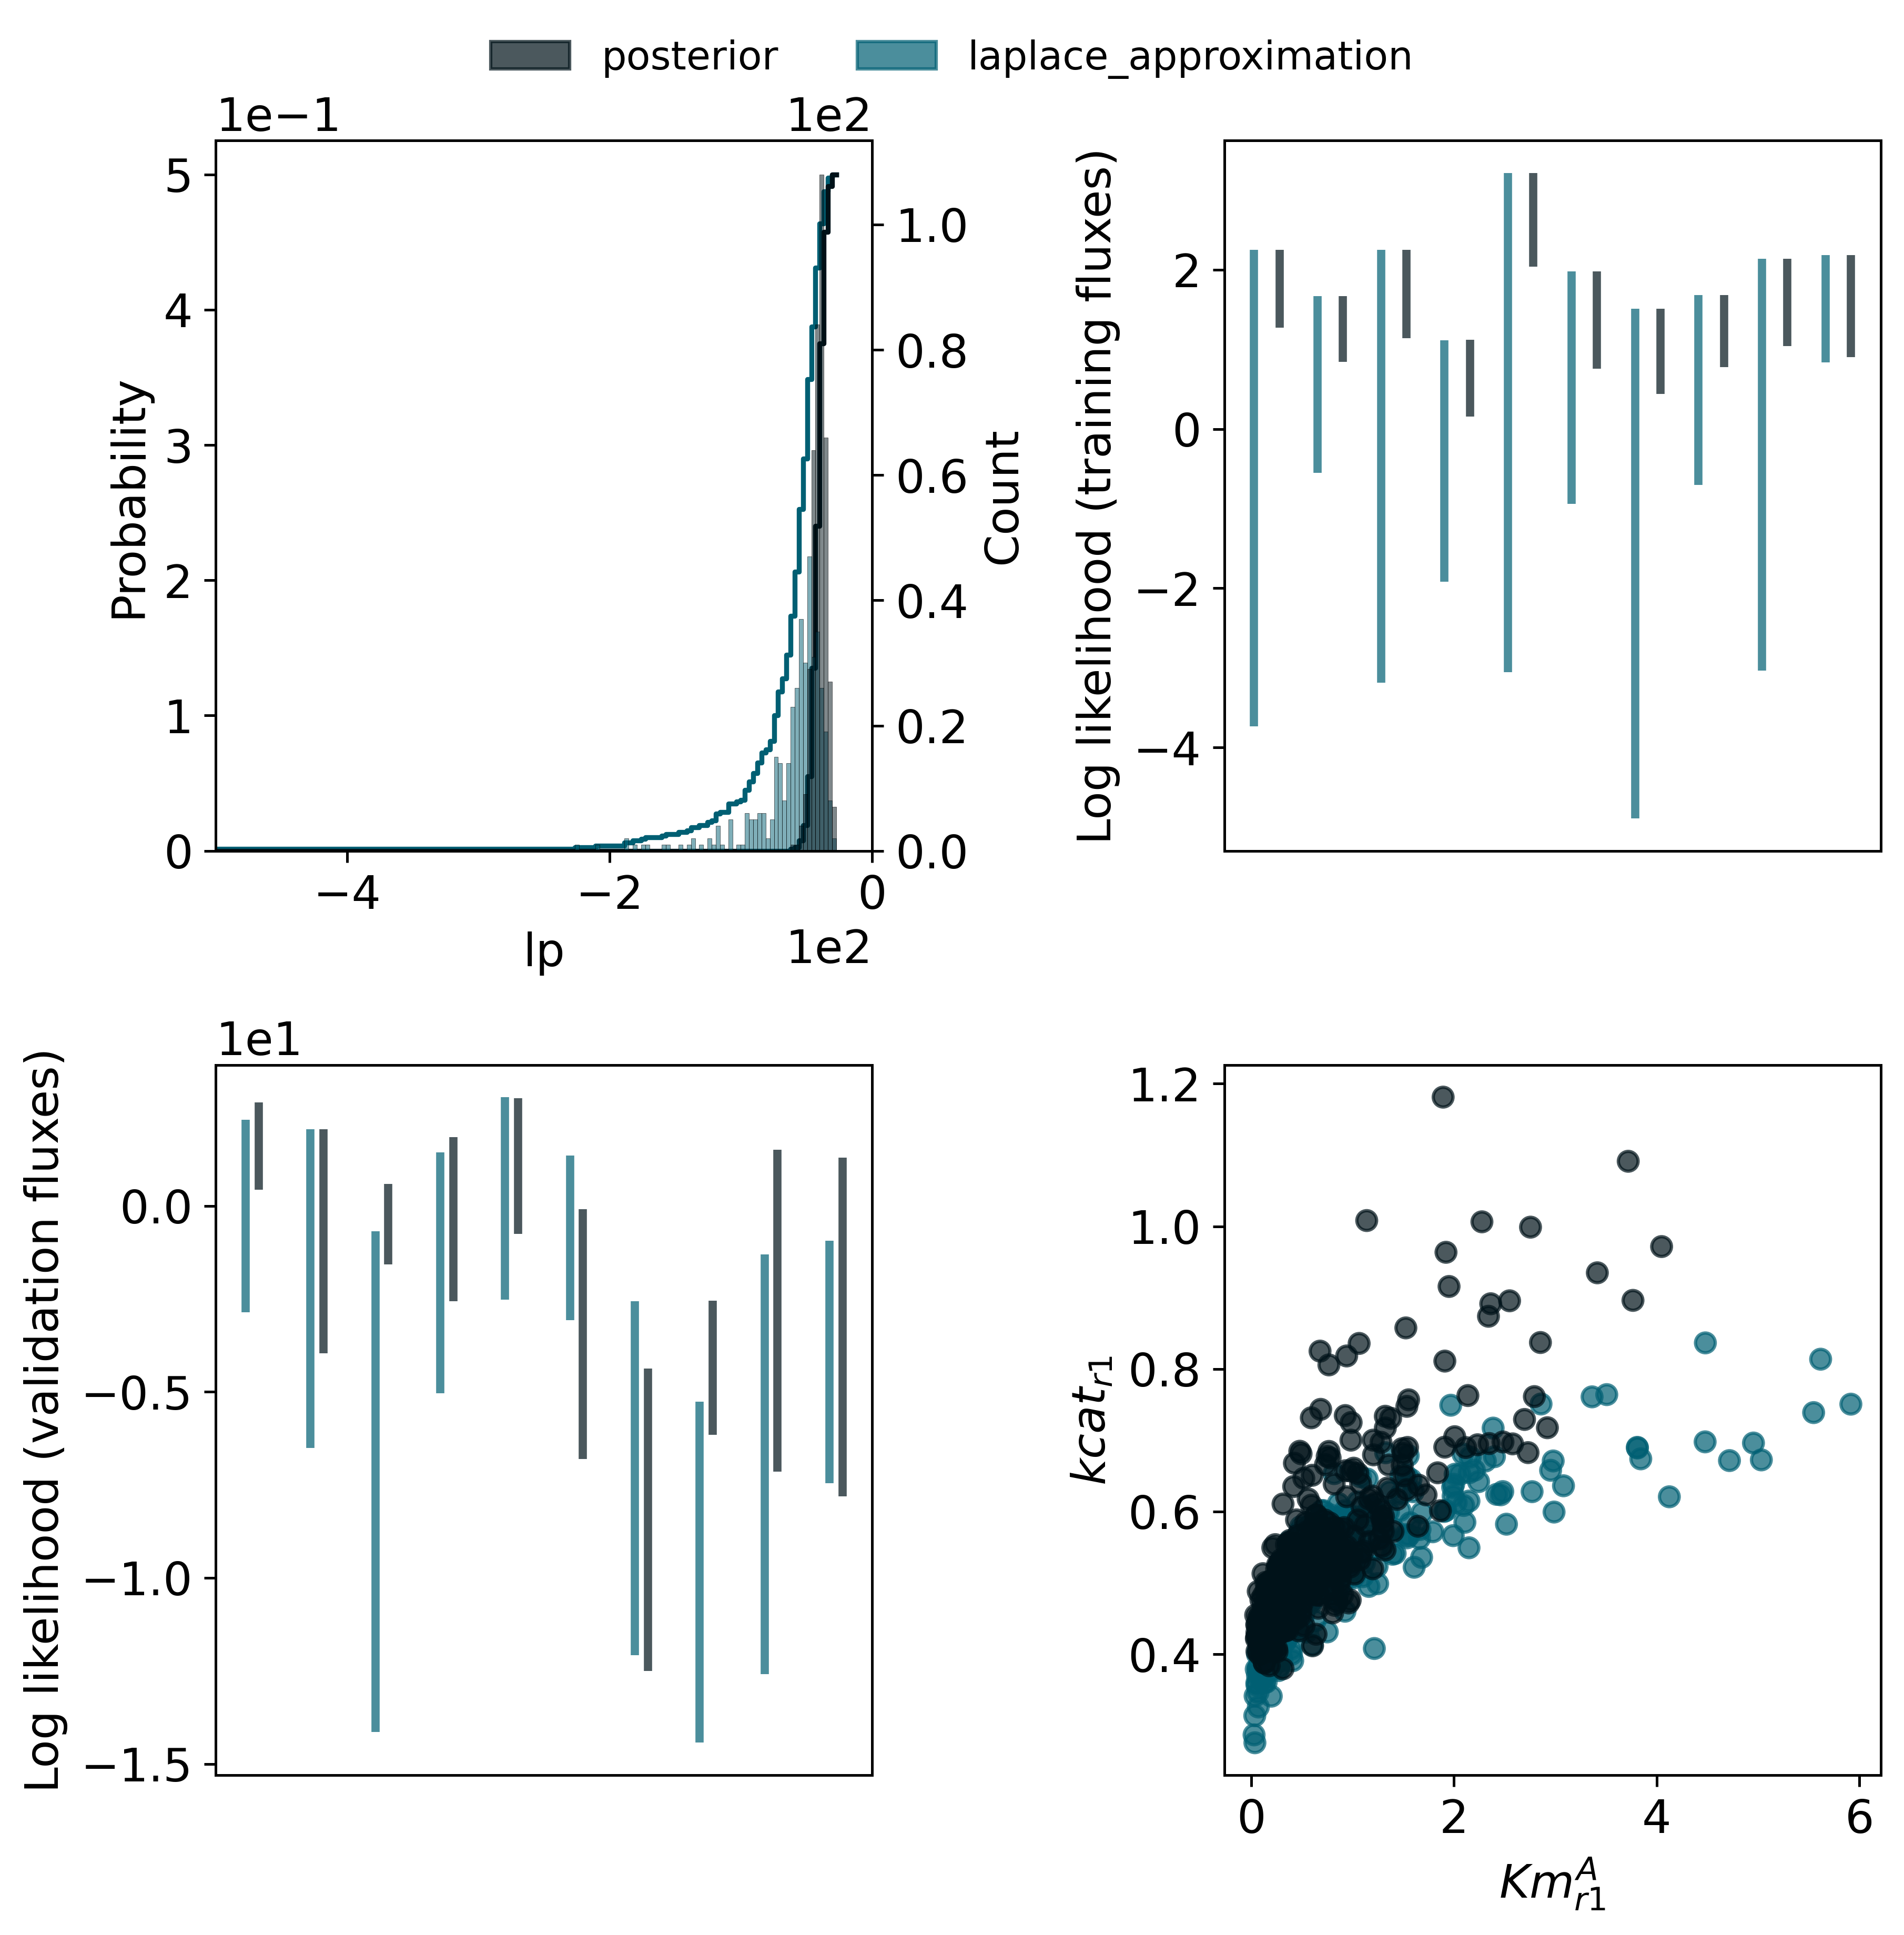
\includegraphics{./figures/laplace.png}

}

\caption{\label{fig-laplace}CAPTION: FILL THIS IN!}

\end{figure}

\hypertarget{effect-of-missing-metabolite-concentration-measurements}{%
\subsubsection{Effect of missing metabolite concentration
measurements}\label{effect-of-missing-metabolite-concentration-measurements}}

Comparing model runs with and without the ahcys measurements showed that
Maud can produce sensible results even from incomplete metabolomics
data.

Figure~\ref{fig-missing} shows that, as might be expected, the model
with missing measurements did not correctly infer the missing ahcys
concentrations. Nonetheless, the remaining measured metabolites were
still well predicted, suggesting that information about the network is
still preserved despite the missing measurements. Comparison of flux
measurements in both models also indicated that removing the ahcys
measurement did not result in catastrophic model failure.

The missing measurements did affect Maud's ability to infer parameter
values correctly. As we can see in the \#lower left plot
of~\ref{fig-missing}, the model with full metabolomics learned the true
value for the displayed dissociation constant, despite this value being
far from the mean of the corresponding marginal prior distribution,
whereas the model with the missing measurements stayed in the
neighbourhood of the prior.

This result is reassuring because not having access to all measurements
is a common situation in multi-omics studies. For instance, measuring
all metabolites in a pathway can be infeasible because of limitations of
mass spectrometers, availability of standards, column effects, and
compartmentalisation. However, provided that sufficient information is
available from other sources, our approach can produce sensible results
from incomplete metabolomics data.

\begin{figure}

{\centering 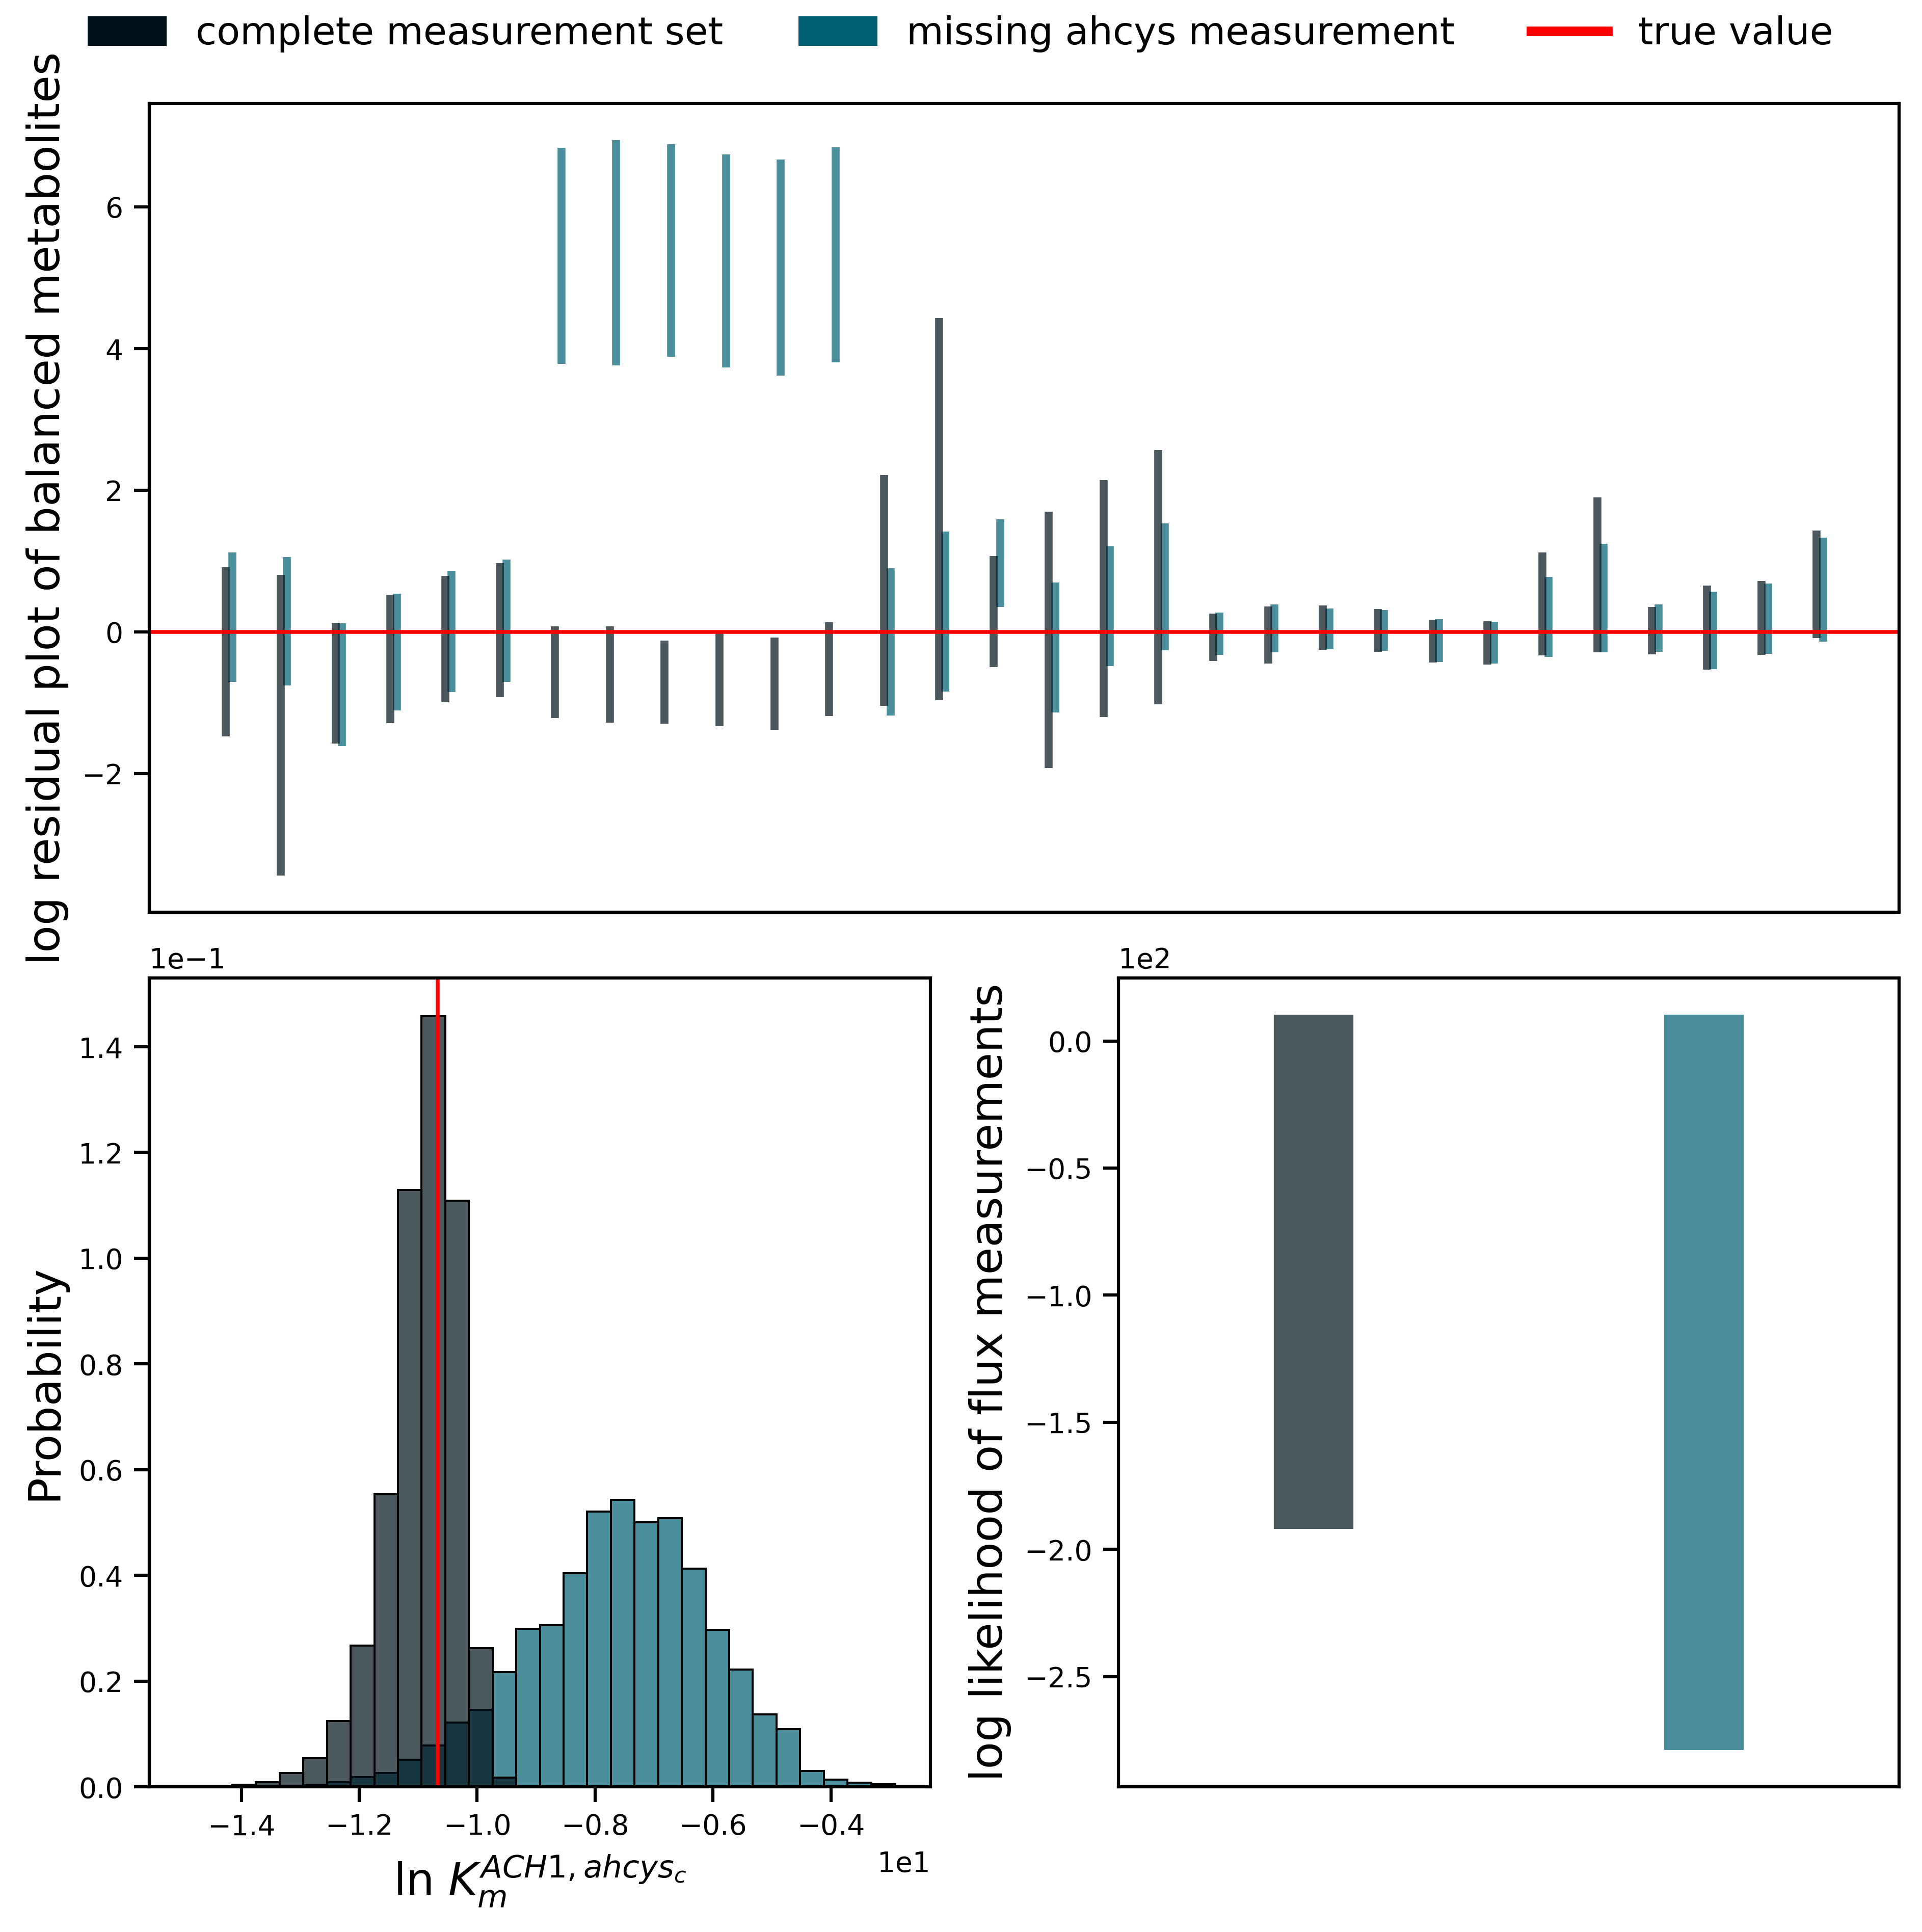
\includegraphics{./figures/missing.png}

}

\caption{\label{fig-missing}CAPTION: FILL THIS IN!}

\end{figure}

\hypertarget{application-to-regulatory-understanding}{%
\subsubsection{Application to regulatory
understanding}\label{application-to-regulatory-understanding}}

To investigate how the flux of GNMT between conditions {[}X{]} and
{[}Y{]} changes we compared the regulatory contributions in the
posterior distribution. Presented in Figure~\ref{fig-decomposition} is
the regulatory description of GNMT, an irreversible enzyme that is
homotropically activated by its substrate, competitively inhibited by
its product and heterotropically inhibited. The diverse regulation makes
it the ideal test case to elucidate regulatory changes.

Here we found that saturation and allosteric effects were the main
drivers of regulation between the two conditions.
Figure~\ref{fig-decomposition} shows the distributions of the regulatory
components as the log-ratio of each component with {[}X{]} in the
numerator and {[}Y{]} in the denominator, positive values suggest that
this component was increased in experiment {[}X{]} relative to {[}Y{]},
with 0 indicating no difference. Naturally, this presents the ideal
statistical test when evaluating the regulation, with the probability of
regulation given by the relative proportion of samples above and below
the 0 point.

We demonstrate that Maud can accurately reproduce the regulatory effect
between the two conditions by comparing it to the ground truth. As the
true values are well within our probability mass of the posterior we can
say that Maud is able to accurately reproduce the regulatory behaviour
of metabolic networks and also provides a tool for statistical inference
of the regulatory behaviour.

Here we have demonstrated a key feature in Maud, that is, direct
inference on any parameter that arises from the data generating process.
More succinctly, we show the benefit of error propagation that Bayesian
inference provides as researchers can directly use quantiles for
hypothesis testing.

Our tool allows inference directly on the joint posterior distribution
rather than the marginal parameter. The implication is that inference
will be better than that of the marginal distributions due to correlated
parameter values, if the data generating process can be directly
modelled.

\begin{figure}

{\centering 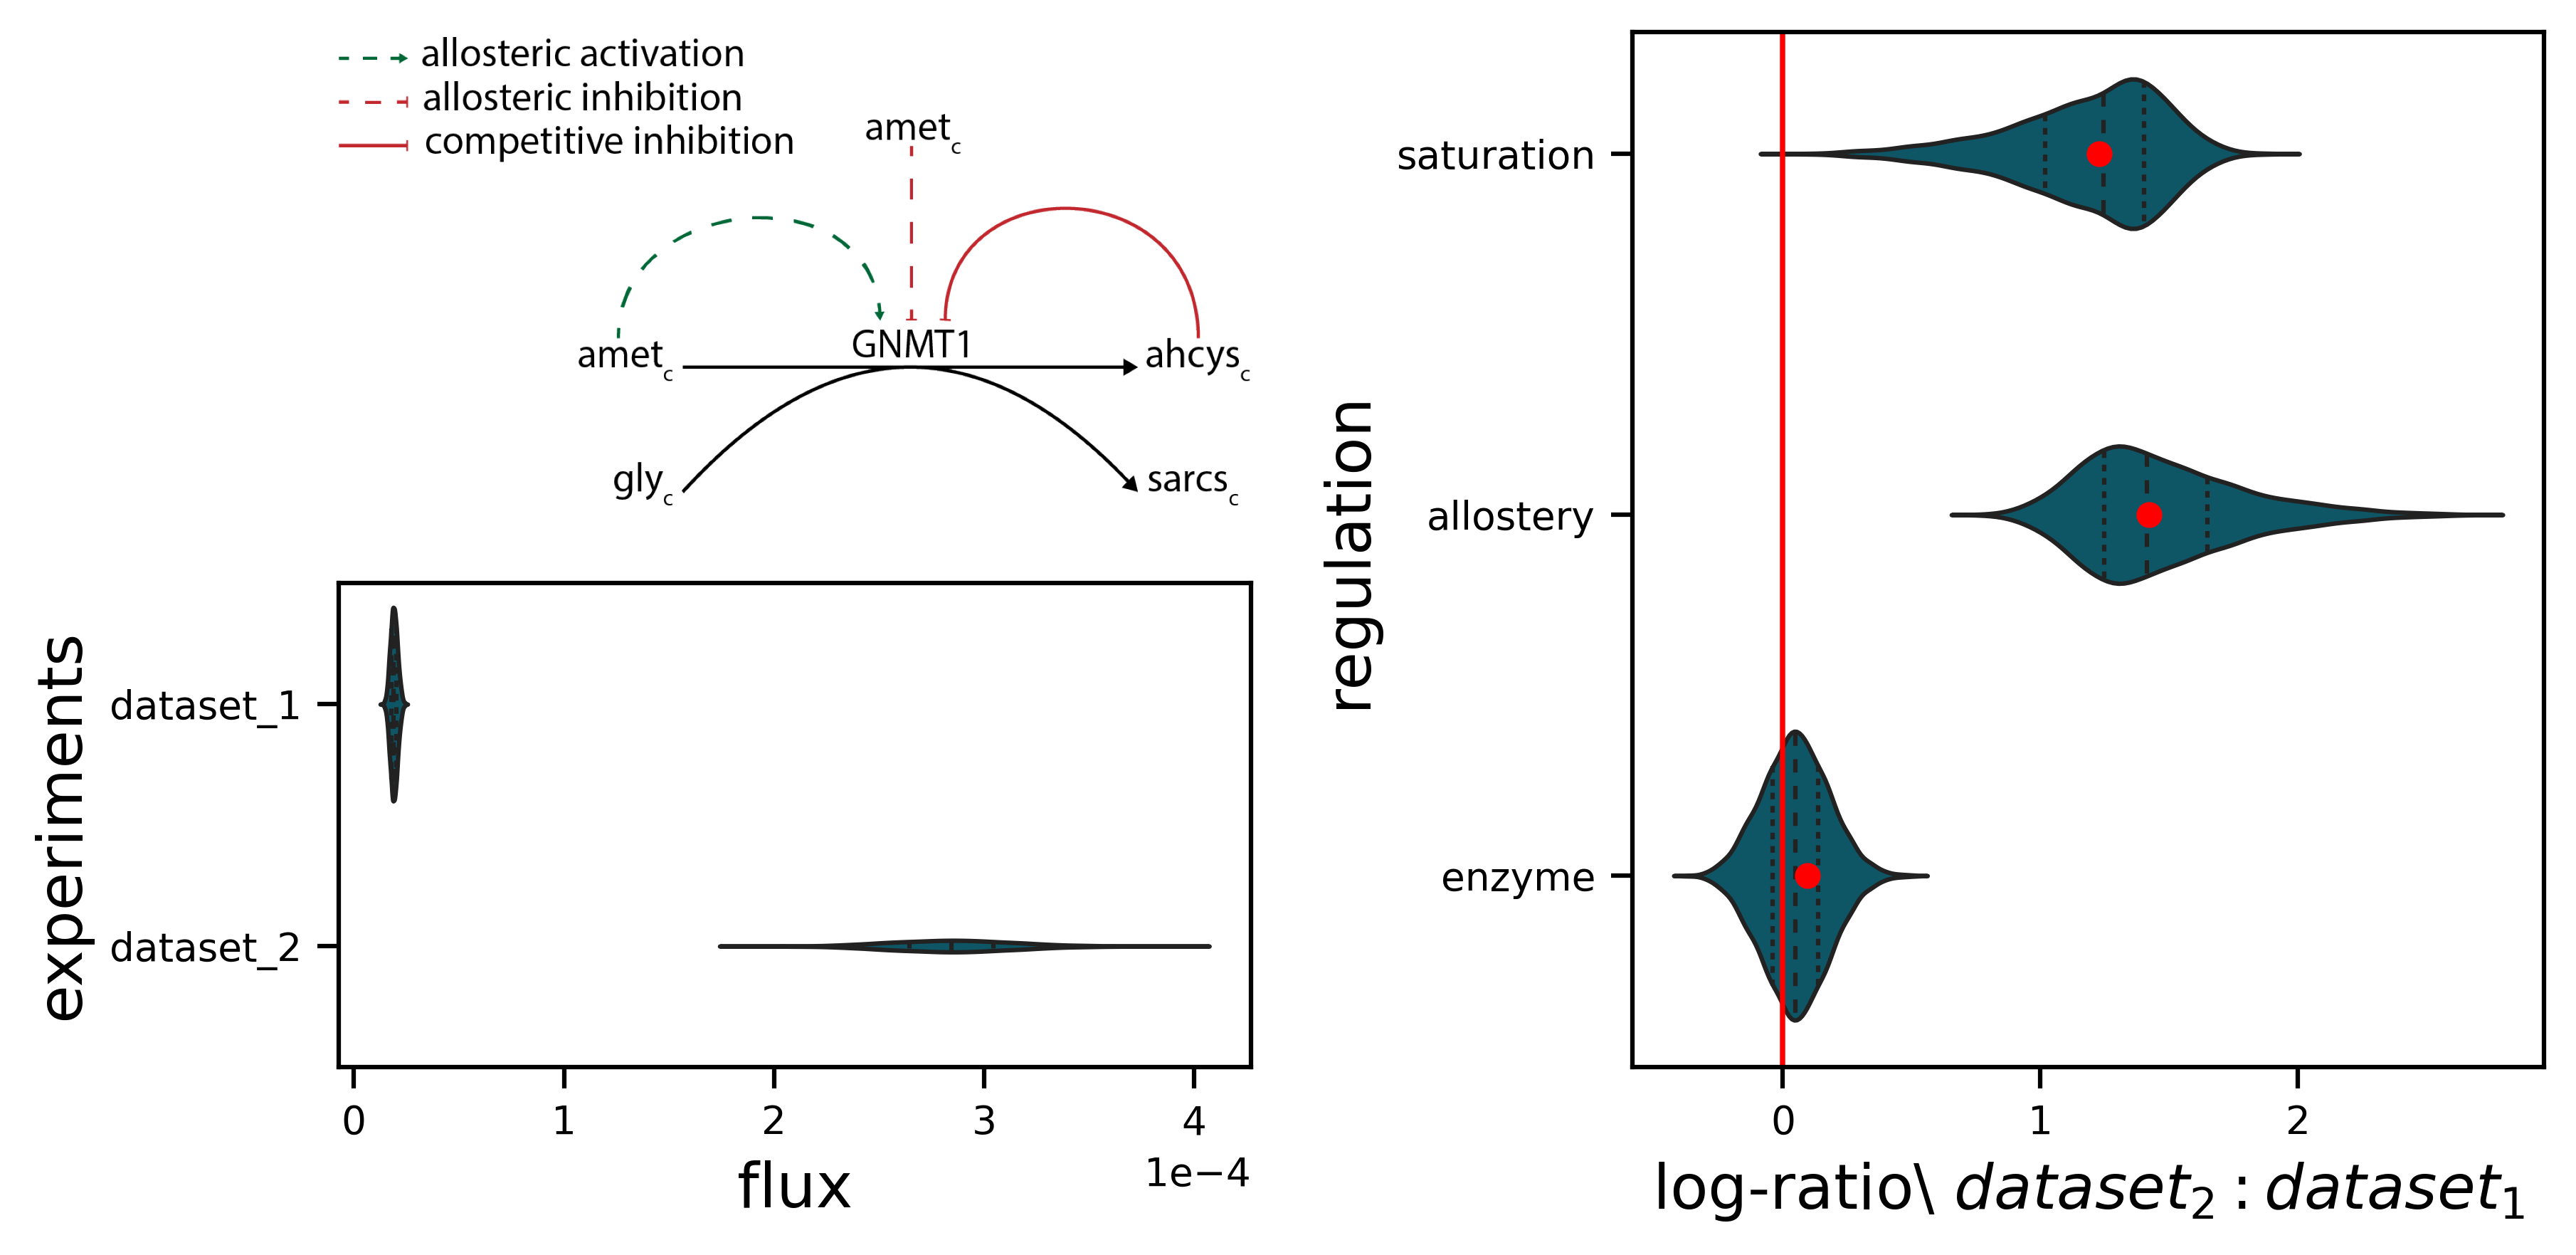
\includegraphics{./figures/decomposition.png}

}

\caption{\label{fig-decomposition}CAPTION: FILL THIS IN!}

\end{figure}

\hypertarget{methods}{%
\section{Methods}\label{methods}}

Maud is a command line application implementing Bayesian inference for a
wide range of realistic kinetic models. Maud is written in Python (Van
Rossum and Drake 2009), designed for use on Windows, Macos and Linux,
registered on the Python Package Index as
\texttt{maud-metabolic-models}, documented at \textless https://maud-
metabolic-models.readthedocs.io\textgreater{} and actively developed and
maintained at \url{https://github.com/biosustain/Maud/}.

To use Maud, a user must first collate appropriate input information,
represent it in files with Maud's required formats (see section
(REFERENCE)below). Maud's command line interface provides commands for
inference, simulation and making out-of-sample predictions. Results are
stored in files, using a structured, interoperable format.

\hypertarget{input-format}{%
\subsection{Input format}\label{input-format}}

Maud inputs are structured directories, somewhat inspired by the PEtab
format Schmiester et al. (2021). A Maud input directory must contain a
toml (Preston-Werner, Tom and Gedam, Pradyun 2020) file called
\texttt{config.toml} which gives the input a name, configures how Maud
will be run and tells Maud where to find the other files, allowing these
to have custom names. It must also include a file containing a kinetic
model definition, a file specifying information about parameters and a
file with information experiments. The required structure of these files
is documented at \textless https://
maud-metabolic-models.readthedocs.io/en/latest/inputting.html\textgreater.
The input is validated against a Pydantic (Pydantic developers 2022)
data model which can be inspected at
\url{https://github.com/biosustain/Maud/tree/main/maud/data_model}.

We chose to implement a custom input format despite the existence of
standard formats in similar areas, including SBML (Keating et al. 2020)
and PEtab (Schmiester et al. 2021). This choice was partly motivated by
the need to ensure flexibility as Maud was developed, but there are also
features of SBML and PEtab that make them structurally unsuitable in
this context. Our requirements for an input format included that it be
mathematics-free, so that all mathematical details are encapsulated in
source code, and that it has a detailed, verifiable structure. These
requirements made toml more attractive than SBML: toml is easier for
humans to read and edit and can straightforwardly be validated using
tools like pydantic. Further, an SBML representation of our desired
input would not contain differential equations. It would therefore not
be interoperable with most SBML-targeting software, which typically
assumes that differential equations are available and does not know
about Maud's structure.

\hypertarget{kinetic-model}{%
\subsection{Kinetic model}\label{kinetic-model}}

Maud's kinetic model decomposes into factors as shown in equation
\eqref{eq-decomposition}.

\begin{equation}
F(C;\theta) = Enzyme\cdot k_{cat}\cdot Reversibility \cdot Saturation \cdot Allostery \label{eq-decomposition}
\end{equation}

Each of the terms on the right-hand side of (REFER TO EQUATION) is a
function of \(C\) and \(\theta\). This idea is taken from Noor et al.
(2013). The terms usefully gather physically meaningful and conceptually
distinct factors contributing to reaction fluxes. \(Enzyme\) captures
the effect of enzyme concentration, \(k_{cat}\) that of enzyme
efficiency, \(Reversibility\) quantifies thermodynamic effects,
\(Saturation\) the effect of enzyme availability and \(Allostery\) the
effect of post translational modifications.

We used the model of enzyme saturation from Liebermeister, Uhlendorf,
and Klipp (2010) and the generalised Monod-Wyman-Changeux model of
Allosteric regulation introduced in (Monod, Wyman, and Changeux 1965;
Changeux 2013; Popova and Sel'kov 1975, 1979) and used more recently in
Matos et al. (2022). To capture the effect on enzyme activity of coupled
phosphorylation and dephosphorylation processes we developed a new
mathematical model inspired by the generalised MWC model of allosteric
regulation. Full details of all mathematical aspects of Maud's kinetic
model can be found in supplementary material section (REFERENCE).

\hypertarget{statistical-model}{%
\subsection{Statistical model}\label{statistical-model}}

Maud represents information from measurements using generalised linear
regression models that probabilistically connect realised measurements
with true values of the measurable quantities. Information from other
sources is represented using a prior distribution over a set of latent
parameters. The parameters and the measurable quantities are connected
by a generative model encompassing Maud's kinetic model as well as the
steady state equation \eqref{eq-3}. Together, the measurement model,
prior model and generative model determine a joint probability function
that assigns a probability density to any possible combination of
measurements and parameters.

Below we describe the prior and measurement models, as the generative
model has already been discussed above.

\hypertarget{prior-model}{%
\subsubsection{Prior model}\label{prior-model}}

Maud's prior model includes unknown parameters corresponding to
quantities in the kinetic model that are assumed to be unknown, other
than steady state metabolite concentrations and fluxes, which are
derived from the values of other parameters by solving the steady state
problem. See Table 1 (REFERENCE) for a description of all these
parameters and their dimensions. Note that some quantities in Maud's
kinetic model are not treated as parameters: for example, temperatures,
compartment volumes and the formation energy of water. Maud treats these
quantities as if they were known precisely: they can be configured by
the user or default values can be used. Although in practice there can
be considerable uncertainty regarding these quantities, we chose to
disregard this uncertainty in the interest of simplicity.

Except for metabolites' standard condition Gibbs energy changes of
formation, Maud uses independent normal prior distributions for
parameters that can in principle be both negative and positive. For
parameters that are constrained to be positive, Maud uses independent
log-normal distributions. Formation energy parameters have a
multivariate normal prior distribution. Location, scale and covariance
parameters for all these prior distributions can be chosen freely by the
user.

\hypertarget{measurement-model-1}{%
\subsubsection{Measurement model}\label{measurement-model-1}}

Maud's measurement model considers three types of measurement:
metabolite concentration measurements, enzyme concentration measurements
and flux measurements, represented by vectors \(𝑦_{𝑐𝑜𝑛𝑐}\) \(𝑦_{𝑒𝑛𝑧}\)
and \(𝑦_{𝑓𝑙𝑢𝑥}\) respectively.

All measurements are specific to an experimental condition - that is, a
case where the true state of the network, including knockouts, boundary
conditions and state variables as well as kinetic and thermodynamic
parameters, can safely be assumed to be the same. Maud's statistical
model allows for arbitrarily many experimental conditions, and for any
measurable quantity to be measured any number of times in any condition.

Metabolite and enzyme measurements are intended to represent the results
of quantitative metabolomics and proteomics experiments. The likelihood
functions for such measurements are shown in equations Equation\,6 and
Equation\,7.

EQUATIONS

Both equations are log-normal generalised linear models with a standard
link function (the natural logarithm \(\ln\)) and known standard
deviation \$ \sigma\_\{𝑐𝑜𝑛𝑐\}\$. The use of this measurement model is
motivated by the consideration that concentrations are constrained to be
non-negative, so the measurement model should avoid assigning positive
probability mass to negative metabolite concentration values. In
addition, we expect the precision of most metabolomics and proteomics
experiments to be roughly proportional to the value of the true measured
quantity, which supports a measurement model with constant coefficient
of variation. The measurement standard deviations \(\sigma_{𝑐𝑜𝑛𝑐}\) and
\(\sigma_{𝑒𝑛𝑧}\) are assumed to be known exactly for simplicity;
plausible values can be elicited by considering the likely coefficient
of variation of the measuring apparatus.

Flux measurements, representing the results of quantitative fluxomics
analyses, are modelled using a likelihood function from a standard
linear regression model, as shown in equation Equation\,8 (REFERENCE).
Flux measurements can be obtained from the results of isotope labelling
experiments using metabolic flux analysis, for example as described in
(Young 2014). When entering flux measurements, it is important only to
specify measurements for a network's free fluxes, as the values of some
steady state fluxes in a metabolic network are constrained by others,
with the result that dependent fluxes cannot typically be measured
separately. If measurements of multiple dependent fluxes are entered,
information will inappropriately be double counted.

EQUATION

Our measurement model improves on analyses of metabolomics and
proteomics data that assume a regression model with normally distributed
errors, whether explicitly using a standard linear model or implicitly
using ordinary least squares fitting. This assumption is undesirable
because it implies that the measured quantity could in principle be
negative, and assumes an additive underlying random process, whereas
multiplicative processes tend to better describe real concentration
data.

The use of independent measurement models for metabolite, enzyme and
flux measurements carries an implicit assumption that there are no
systematic correlations in the measurement errors. This choice was
motivated by simplicity - it would be better to use a model with
potentially correlated measurements. Similarly, it would be preferable
to include measurement errors as model parameters, thereby avoiding
possible bias due to incorrect assessments of measurement accuracy.
However, we chose to use a simpler measurement model to avoid the
complexity and potential fitting issues that these changes would entail.

Finally, the reader may wonder why we chose a linear regression model
for reaction flux measurements even though this creates the potential
for erroneous double counting and requires non-trivial upstream
modelling, as intracellular fluxes typically cannot be measured
directly, but must be inferred from isotope labelling experiments using
metabolic flux analysis (see REFERENCE). Ideally Maud's measurement
model for fluxes would extend from fluxes to the results of potential
labelling experiments, thereby removing the need for upstream analysis
and avoiding any double counting. This option has not yet been pursued,
again for the sake of simplicity.

\hypertarget{implementation}{%
\subsection{Implementation}\label{implementation}}

Maud uses the Python library click (Click Developers 2022) to implement
a command line interface. The command line interface loads input files
as Python dictionaries, which are parsed using the Python library
\texttt{toml} (Pearson 2020) and then validated and converted into
structured \texttt{MaudInput} objects using Pydantic (Pydantic
developers 2022). Maud's statistical model is implemented in the
probabilistic programming language Stan (Carpenter et al. 2017) and
accessed using the interface cmdstanpy (Stan Development Team 2022). For
posterior sampling, Maud uses the \texttt{MaudInput} to create a Stan
input json file and obtain configuration information for cmdstanpy,
which it uses to (if necessary) generate a model executable file and
then trigger posterior sampling using adaptive Hamiltonian Monte Carlo.
When sampling is complete, Maud converts to the output into the standard
format InferenceData using the Python library arviz (Kumar et al. 2019)
and saves it as a json file, along with some information for debugging.

Two details of Maud's implementation are important to highlight: the
method of posterior sampling and how Maud solves the steady state
problem \eqref{eq-3}.

\hypertarget{posterior-sampling}{%
\subsubsection{Posterior sampling}\label{posterior-sampling}}

Although integrals of the joint probability model for kinetic models are
typically analytically intractable, they can be approximated numerically
using Markov Chain Monte Carlo (MCMC) and other methods. Maud uses MCMC
primarily because there exist many methods for verifying that MCMC
samples really do approximate the target probability distribution:
see@vehtariRankNormalizationFoldingLocalization2021 and Talts et al.
(2018) for discussion of this point. In addition, there are several
examples of successful Bayesian kinetic modelling projects using MCMC
including St. John et al. (2018) and Xing et al. (2010 Jan-Feb).

\hypertarget{solving-the-steady-state-problem}{%
\subsubsection{Solving the steady state
problem}\label{solving-the-steady-state-problem}}

In order to implement adaptive Hamiltonian Monte Carlo, Maud must
repeatedly solve the steady state problem \eqref{eq-3} and find its
gradients with respect to all parameters. To achieve this, Maud uses a
hybrid method involving two numerical solvers from the SUNDIALS suite
(Serban and Hindmarsh 2005): CVODES and IDAS. These solvers are accessed
via their interface from Stan. The hybrid method follows that propsed by
Margossian (2018), and involves numerically evolving the ODE system for
a short period of time, then using the difference between the evolved
and starting concentrations as the target for a numerical algebra
solver.

\hypertarget{acknowledgements}{%
\section{Acknowledgements}\label{acknowledgements}}

\hypertarget{references}{%
\section{References}\label{references}}

\hypertarget{refs}{}
\begin{CSLReferences}{1}{0}
\leavevmode\vadjust pre{\hypertarget{ref-carpenterStanProbabilisticProgramming2017}{}}%
Carpenter, Bob, Andrew Gelman, Matthew D. Hoffman, Daniel Lee, Ben
Goodrich, Michael Betancourt, Marcus Brubaker, Jiqiang Guo, Peter Li,
and Allen Riddell. 2017. {``Stan: {A Probabilistic Programming
Language}.''} \emph{Journal of Statistical Software} 76 (1): 1--32.
\url{https://doi.org/10.18637/jss.v076.i01}.

\leavevmode\vadjust pre{\hypertarget{ref-changeux_2013}{}}%
Changeux, Jean-Pierre. 2013. {``50 Years of Allosteric Interactions: The
Twists and Turns of the Models.''} \emph{Nature Reviews. Molecular Cell
Biology} 14 (12): 819--29. \url{https://doi.org/10.1038/nrm3695}.

\leavevmode\vadjust pre{\hypertarget{ref-christodoulou_reserve_2018}{}}%
Christodoulou, Dimitris, Hannes Link, Tobias Fuhrer, Karl Kochanowski,
Luca Gerosa, and Uwe Sauer. 2018. {``Reserve {Flux} {Capacity} in the
{Pentose} {Phosphate} {Pathway} {Enables} {Escherichia} Coli's {Rapid}
{Response} to {Oxidative} {Stress}.''} \emph{Cell Systems} 6 (5):
569--578.e7. \url{https://doi.org/10.1016/j.cels.2018.04.009}.

\leavevmode\vadjust pre{\hypertarget{ref-clickdevelopersClickPythonComposable2022}{}}%
Click Developers. 2022. {``Click: {Python} Composable Command Line
Interface Toolkit.''} Pallets. \url{https://pypi.org/project/click/}.

\leavevmode\vadjust pre{\hypertarget{ref-deberardinis_fundamentals_2016}{}}%
DeBerardinis, Ralph J, and Navdeep S Chandel. 2016. {``Fundamentals of
Cancer Metabolism.''} \emph{Science Advances} 2 (5): e1600200.
\url{https://doi.org/10.1126/sciadv.1600200}.

\leavevmode\vadjust pre{\hypertarget{ref-gopalakrishnan_k-fit_2020}{}}%
Gopalakrishnan, Saratram, Satyakam Dash, and Costas Maranas. 2020.
{``K-{FIT}: {An} Accelerated Kinetic Parameterization Algorithm Using
Steady-State Fluxomic Data.''} \emph{Metabolic Engineering}, March.
\url{https://doi.org/10.1016/j.ymben.2020.03.001}.

\leavevmode\vadjust pre{\hypertarget{ref-gutenkunst_2007}{}}%
Gutenkunst, Ryan N, Joshua J Waterfall, Fergal P Casey, Kevin S Brown,
Christopher R Myers, and James P Sethna. 2007. {``Universally Sloppy
Parameter Sensitivities in Systems Biology Models.''} \emph{PLoS
Computational Biology} 3 (10): 1871--78.
\url{https://doi.org/10.1371/journal.pcbi.0030189}.

\leavevmode\vadjust pre{\hypertarget{ref-keatingSBMLLevelExtensible2020}{}}%
Keating, Sarah M, Dagmar Waltemath, Matthias König, Fengkai Zhang,
Andreas Dräger, Claudine Chaouiya, Frank T Bergmann, et al. 2020.
{``{\textsc{SBML}} {Level} 3: An Extensible Format for the Exchange and
Reuse of Biological Models.''} \emph{Molecular Systems Biology} 16 (8):
e9110. \url{https://doi.org/10.15252/msb.20199110}.

\leavevmode\vadjust pre{\hypertarget{ref-korendyaseva_allosteric_2008}{}}%
Korendyaseva, Tatyana K., Denis N. Kuvatov, Vladimir A. Volkov, Michael
V. Martinov, Victor M. Vitvitsky, Ruma Banerjee, and Fazoil I.
Ataullakhanov. 2008. {``An {Allosteric} {Mechanism} for {Switching}
Between {Parallel} {Tracks} in {Mammalian} {Sulfur} {Metabolism}.''}
Edited by Daniel Segre. \emph{PLoS Computational Biology} 4 (5):
e1000076. \url{https://doi.org/10.1371/journal.pcbi.1000076}.

\leavevmode\vadjust pre{\hypertarget{ref-kumarArviZUnifiedLibrary2019}{}}%
Kumar, Ravin, Colin Carroll, Ari Hartikainen, and Osvaldo Martin. 2019.
{``{ArviZ} a Unified Library for Exploratory Analysis of {Bayesian}
Models in {Python}.''} \emph{Journal of Open Source Software} 4 (33):
1143. \url{https://doi.org/10.21105/joss.01143}.

\leavevmode\vadjust pre{\hypertarget{ref-Liberti2017}{}}%
Liberti, Maria V., Ziwei Dai, Suzanne E. Wardell, Joshua A. Baccile,
Xiaojing Liu, Xia Gao, Robert Baldi, et al. 2017. {``A {Predictive}
{Model} for {Selective} {Targeting} of the {Warburg} {Effect} Through
{GAPDH} {Inhibition} with a {Natural} {Product}.''} \emph{Cell
Metabolism} 26 (4): 648--659.e8.
\url{https://doi.org/10.1016/j.cmet.2017.08.017}.

\leavevmode\vadjust pre{\hypertarget{ref-liebermeister_model_2021}{}}%
Liebermeister, Wolfram, and Elad Noor. 2021. {``Model {Balancing}: {A}
{Search} for {In}-{Vivo} {Kinetic} {Constants} and {Consistent}
{Metabolic} {States}.''} \emph{Metabolites} 11 (11): 749.
\url{https://doi.org/10.3390/metabo11110749}.

\leavevmode\vadjust pre{\hypertarget{ref-liebermeister_modular_2010}{}}%
Liebermeister, Wolfram, Jannis Uhlendorf, and Edda Klipp. 2010.
{``Modular Rate Laws for Enzymatic Reactions: Thermodynamics,
Elasticities and Implementation.''} \emph{Bioinformatics} 26 (12):
1528--34. \url{https://doi.org/10.1093/bioinformatics/btq141}.

\leavevmode\vadjust pre{\hypertarget{ref-margossianComputingSteadyStates2018}{}}%
Margossian, Charles. 2018. {``Computing Steady States with {Stan}'s
Nonlinear Algebraic Solver.''} In \emph{Stan {Conference} 2018}.
\url{https://doi.org/10.5281/zenodo.1284375}.

\leavevmode\vadjust pre{\hypertarget{ref-matosGRASPComputationalPlatform2022}{}}%
Matos, Marta R A, Pedro A Saa, Nicholas Cowie, Svetlana Volkova, Marina
de Leeuw, and Lars K Nielsen. 2022. {``{GRASP}: A Computational Platform
for Building Kinetic Models of Cellular Metabolism.''}
\emph{Bioinformatics Advances} 2 (1): vbac066.
\url{https://doi.org/10.1093/bioadv/vbac066}.

\leavevmode\vadjust pre{\hypertarget{ref-monod_nature_1965}{}}%
Monod, J, J Wyman, and J P Changeux. 1965. {``On the Nature of
Allosteric Transitions: A Plausible Model.''} \emph{Journal of Molecular
Biology} 12 (May): 88--118.
\url{https://doi.org/10.1016/S0022-2836(65)80285-6}.

\leavevmode\vadjust pre{\hypertarget{ref-noor_note_2013}{}}%
Noor, Elad, Avi Flamholz, Wolfram Liebermeister, Arren Bar-Even, and Ron
Milo. 2013. {``A Note on the Kinetics of Enzyme Action: {A}
Decomposition That Highlights Thermodynamic Effects.''} \emph{FEBS
Letters}, A century of {Michaelis} - {Menten} kinetics, 587 (17):
2772--77. \url{https://doi.org/10.1016/j.febslet.2013.07.028}.

\leavevmode\vadjust pre{\hypertarget{ref-pearsonTomlPythonLibrary2020}{}}%
Pearson, William. 2020. {``Toml: {Python Library} for {Tom}'s {Obvious},
{Minimal Language}.''} \url{https://pypi.org/project/toml/}.

\leavevmode\vadjust pre{\hypertarget{ref-poirier_revising_1998}{}}%
Poirier, Dale J. 1998. {``{REVISING} {BELIEFS} {IN} {NONIDENTIFIED}
{MODELS}.''} \emph{Econometric Theory} 14 (4): 483--509.
\url{https://doi.org/10.1017/S0266466698144043}.

\leavevmode\vadjust pre{\hypertarget{ref-popova_generalization_1975}{}}%
Popova, S V, and E E Sel'kov. 1975. {``Generalization of the Model by
{Monod}, {Wyman} and {Changeux} for the Case of a Reversible
Monosubtrate Reaction {SR},{TP}.''} \emph{FEBS Letters} 53 (3): 269--73.
\url{https://doi.org/10.1016/0014-5793(75)80034-2}.

\leavevmode\vadjust pre{\hypertarget{ref-popova_description_1979}{}}%
---------. 1979. {``{[}{Description} of the Kinetics of the Two
Substrate Reactions {S1}+{S2} Goes to and Comes from {S3}+{S4} by a
Generalized {Monod}, {Wyman}, {Changeux} Model{]}.''}
\emph{Molekuliarnaia Biologiia} 13 (1): 129--39.
\url{https://www.ncbi.nlm.nih.gov/pubmed/156878}.

\leavevmode\vadjust pre{\hypertarget{ref-preston-wernertomandgedampradyunTOMLSpecification0rc2020}{}}%
Preston-Werner, Tom and Gedam, Pradyun. 2020. {``{TOML Specification}
1.0.0-Rc.1.''} \url{https://toml.io/en/v1.0.0-rc.1/}.

\leavevmode\vadjust pre{\hypertarget{ref-pydanticdevelopersPydantic2022}{}}%
Pydantic developers. 2022. {``Pydantic.''}
\url{https://pypi.org/project/pydantic/}.

\leavevmode\vadjust pre{\hypertarget{ref-raue_identifiability_2010}{}}%
Raue, A., V. Becker, U. Klingmüller, and J. Timmer. 2010.
{``Identifiability and Observability Analysis for Experimental Design in
Nonlinear Dynamical Models.''} \emph{Chaos: An Interdisciplinary Journal
of Nonlinear Science} 20 (4): 045105.
\url{https://doi.org/10.1063/1.3528102}.

\leavevmode\vadjust pre{\hypertarget{ref-raue_joining_2013}{}}%
Raue, Andreas, Clemens Kreutz, Fabian Joachim Theis, and Jens Timmer.
2013. {``Joining Forces of {Bayesian} and Frequentist Methodology: A
Study for Inference in the Presence of Non-Identifiability.''}
\emph{Philosophical Transactions of the Royal Society A: Mathematical,
Physical and Engineering Sciences} 371 (1984): 20110544.
\url{https://doi.org/10.1098/rsta.2011.0544}.

\leavevmode\vadjust pre{\hypertarget{ref-saa_construction_2016}{}}%
Saa, Pedro A, and Lars K Nielsen. 2016. {``Construction of Feasible and
Accurate Kinetic Models of Metabolism: {A} {Bayesian} Approach.''}
\emph{Scientific Reports} 6 (July): 29635.
\url{https://doi.org/10.1038/srep29635}.

\leavevmode\vadjust pre{\hypertarget{ref-saa_general_2015}{}}%
Saa, Pedro, and Lars K Nielsen. 2015. {``A General Framework for
Thermodynamically Consistent Parameterization and Efficient Sampling of
Enzymatic Reactions.''} \emph{PLoS Computational Biology} 11 (4):
e1004195. \url{https://doi.org/10.1371/journal.pcbi.1004195}.

\leavevmode\vadjust pre{\hypertarget{ref-SchmiesterSch2021}{}}%
Schmiester, Leonard, Yannik Schälte, Frank T. Bergmann, Tacio Camba,
Erika Dudkin, Janine Egert, Fabian Fröhlich, et al. 2021.
{``{PEtab}\textemdash{{Interoperable}} Specification of Parameter
Estimation Problems in Systems Biology.''} \emph{PLOS Computational
Biology} 17 (1): 1--10.
\url{https://doi.org/10.1371/journal.pcbi.1008646}.

\leavevmode\vadjust pre{\hypertarget{ref-serbanCVODESSensitivityEnabledODE2005}{}}%
Serban, Radu, and Alan C. Hindmarsh. 2005. {``{CVODES}: {The
Sensitivity-Enabled ODE Solver} in {SUNDIALS}.''} In \emph{Volume 6: 5th
{International Conference} on {Multibody Systems}, {Nonlinear Dynamics},
and {Control}, {Parts A}, {B}, and {C}}, 257--69. {Long Beach,
California, USA}: {ASMEDC}.
\url{https://doi.org/10.1115/DETC2005-85597}.

\leavevmode\vadjust pre{\hypertarget{ref-st.johnBayesianInferenceMetabolic2018}{}}%
St. John, Peter, Jonathan Strutz, Linda J Broadbelt, Keith E J Tyo, and
Yannick J Bomble. 2018. {``Bayesian Inference of Metabolic Kinetics from
Genome-Scale Multiomics Data.''} \emph{bioRxiv}, October.
\url{https://doi.org/10.1101/450163}.

\leavevmode\vadjust pre{\hypertarget{ref-standevelopmentteamCmdStanPy2022}{}}%
Stan Development Team. 2022. {``{CmdStanPy}.''}
\url{https://github.com/stan-dev/cmdstanpy}.

\leavevmode\vadjust pre{\hypertarget{ref-stapor_pesto_2018}{}}%
Stapor, Paul, Daniel Weindl, Benjamin Ballnus, Sabine Hug, Carolin Loos,
Anna Fiedler, Sabrina Krause, et al. 2018. {``{PESTO}: Parameter
Estimation Toolbox.''} \emph{Bioinformatics} 34 (4): 705--7.
\url{https://doi.org/10.1093/bioinformatics/btx676}.

\leavevmode\vadjust pre{\hypertarget{ref-taltsValidatingBayesianInference2018}{}}%
Talts, Sean, Michael Betancourt, Daniel Simpson, Aki Vehtari, and Andrew
Gelman. 2018. {``Validating {Bayesian Inference Algorithms} with
{Simulation-Based Calibration}.''} \emph{arXiv:1804.06788 {[}Stat{]}},
April. \url{http://arxiv.org/abs/1804.06788}.

\leavevmode\vadjust pre{\hypertarget{ref-vanrossumPythonReferenceManual2009}{}}%
Van Rossum, Guido, and Fred L. Drake. 2009. \emph{Python 3 {Reference
Manual}}. {Scotts Valley, CA}: {CreateSpace}.

\leavevmode\vadjust pre{\hypertarget{ref-vehtariRankNormalizationFoldingLocalization2021}{}}%
Vehtari, Aki, Andrew Gelman, Daniel Simpson, Bob Carpenter, and
Paul-Christian Bürkner. 2021. {``Rank-{Normalization}, {Folding}, and
{Localization}: {An Improved R\^{}} for {Assessing Convergence} of
{MCMC} (with {Discussion}).''} \emph{Bayesian Analysis} 16 (2):
667--718. \url{https://doi.org/10.1214/20-BA1221}.

\leavevmode\vadjust pre{\hypertarget{ref-visser_dynamic_2003}{}}%
Visser, Diana, and Joseph J Heijnen. 2003. {``Dynamic Simulation and
Metabolic Re-Design of a Branched Pathway Using Linlog Kinetics.''}
\emph{Metabolic Engineering} 5 (3): 164--76.
\url{https://doi.org/10.1016/s1096-7176(03)00025-9}.

\leavevmode\vadjust pre{\hypertarget{ref-white_2016}{}}%
White, Andrew, Malachi Tolman, Howard D Thames, Hubert Rodney Withers,
Kathy A Mason, and Mark K Transtrum. 2016. {``The Limitations of
Model-Based Experimental Design and Parameter Estimation in Sloppy
Systems.''} \emph{PLoS Computational Biology} 12 (12): e1005227.
\url{https://doi.org/10.1371/journal.pcbi.1005227}.

\leavevmode\vadjust pre{\hypertarget{ref-xingModelingKineticsLargescale2010}{}}%
Xing, Zizhuo, Nikki Bishop, Kirk Leister, and Zheng Jian Li. 2010
Jan-Feb. {``Modeling Kinetics of a Large-Scale Fed-Batch {CHO} Cell
Culture by {Markov} Chain {Monte Carlo} Method.''} \emph{Biotechnology
Progress} 26 (1): 208--19. \url{https://doi.org/10.1002/btpr.284}.

\end{CSLReferences}



\end{document}
